\documentclass[11pt, a4paper]{article}
\usepackage[utf8]{inputenc}
\usepackage{geometry}
\geometry{margin=1in}
\usepackage{graphicx}
\usepackage{enumitem}
\usepackage{float}
\usepackage{xcolor}
\usepackage{tikz}
\usetikzlibrary{shapes.geometric, arrows, positioning}

\title{\textbf{OptiFlow: Spatial Intelligence and Crowd Orchestration System}\\
\large Architecture and Implementation Report}
\author{Project Engineering Team}
\date{\today}

\begin{document}

\maketitle

\begin{abstract}
This report details the design, architecture, and implementation of OptiFlow, a production-grade spatial intelligence and crowd orchestration platform built for high-density venues such as transit hubs, stadiums, and exhibition centers. The system leverages a decoupled, hybrid-edge pipeline, integrating a high-throughput FastAPI backend, a responsive React-based Single Page Application (SPA) dashboard, and an XGBoost machine learning inference engine. By processing real-time telemetry through a deterministic multi-agent pipeline and broadcasting insights over a low-latency WebSocket connection, OptiFlow converts raw camera and sensor data into proactive, autonomous safety routing to mitigate crowd crush risks.
\end{abstract}

\section{Introduction}
Managing extreme crowd density requires transitioning from reactive surveillance to proactive spatial intelligence. OptiFlow was engineered to bridge the gap between edge-computed hardware telemetry and high-level operational decision-making. Utilizing a centralized command dashboard, predictive machine learning regression models, and strict deterministic agent constraints, the platform alerts security personnel to localized bottlenecks and orchestrates automated dispatch instructions before congestion reaches critical thresholds.

\section{System Architecture}
The OptiFlow platform is constructed on a multi-tiered architecture designed for extreme low-latency processing and zero-hallucination reliability.

\begin{figure}[H]
    \centering
    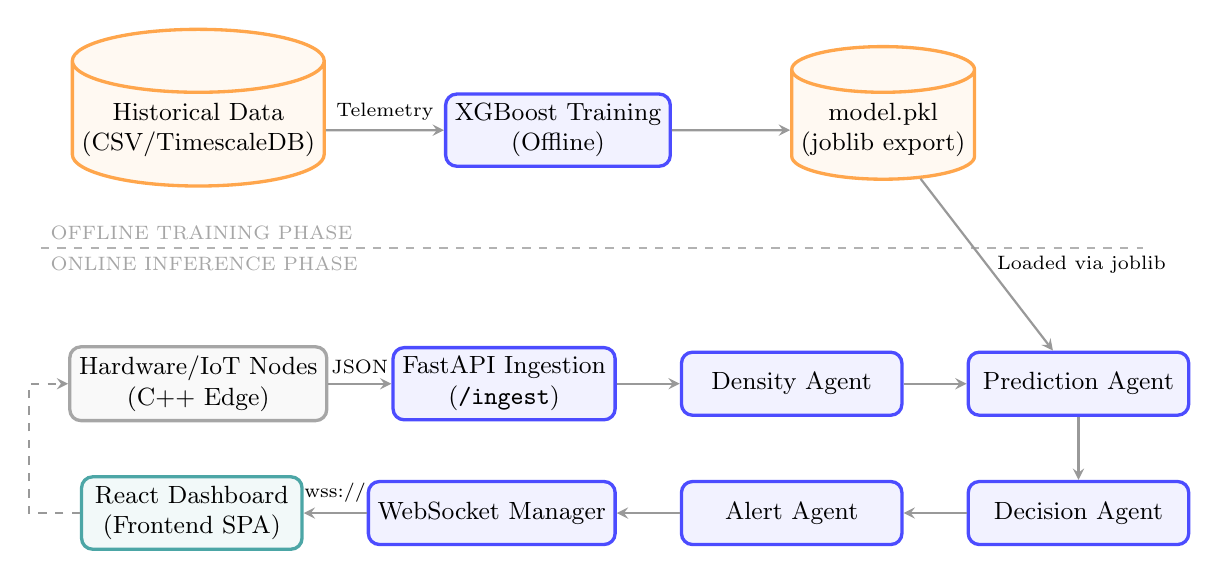
\begin{tikzpicture}[
        node distance=0.8cm and 1cm,
        box/.style={rectangle, draw=blue!70, fill=blue!5, very thick, minimum width=2.8cm, minimum height=0.8cm, align=center, rounded corners, font=\small},
        edgebox/.style={rectangle, draw=gray!70, fill=gray!5, very thick, minimum width=2.8cm, minimum height=0.8cm, align=center, rounded corners, font=\small},
        reactbox/.style={rectangle, draw=teal!70, fill=teal!5, very thick, minimum width=2.8cm, minimum height=0.8cm, align=center, rounded corners, font=\small},
        modelbox/.style={cylinder, draw=orange!70, fill=orange!5, very thick, aspect=0.25, minimum width=2.2cm, minimum height=1cm, align=center, shape border rotate=90, font=\small},
        arrow/.style={-stealth, thick, draw=gray!80}
        ]

        % Offline Training Pipeline (Top)
        \node (db) [modelbox] {Historical Data\\(CSV/TimescaleDB)};
        \node (train) [box, right=1.5cm of db] {XGBoost Training\\(Offline)};
        \node (model) [modelbox, right=1.5cm of train] {model.pkl\\(joblib export)};

        \draw [arrow] (db) -- node[anchor=south, font=\scriptsize] {Telemetry} (train);
        \draw [arrow] (train) -- (model);

        % Separation Line
        \draw [dashed, thick, draw=gray!60] (-2, -1.5) -- (12, -1.5);
        \node [anchor=west, font=\scriptsize, text=gray!70] at (-2, -1.3) {OFFLINE TRAINING PHASE};
        \node [anchor=west, font=\scriptsize, text=gray!70] at (-2, -1.7) {ONLINE INFERENCE PHASE};

        % Online Inference Pipeline (Bottom)
        \node (iot) [edgebox, below=2cm of db] {Hardware/IoT Nodes\\(C++ Edge)};
        \node (ingest) [box, right=0.8cm of iot] {FastAPI Ingestion\\(\texttt{/ingest})};
        
        \node (density) [box, right=0.8cm of ingest] {Density Agent};
        \node (prediction) [box, right=0.8cm of density] {Prediction Agent};
        
        \node (decision) [box, below=0.8cm of prediction] {Decision Agent};
        \node (alert) [box, left=0.8cm of decision] {Alert Agent};
        \node (ws) [box, left=0.8cm of alert] {WebSocket Manager};
        \node (react) [reactbox, left=0.8cm of ws] {React Dashboard\\(Frontend SPA)};

        % Inference arrows
        \draw [arrow] (iot) -- node[anchor=south, font=\scriptsize] {JSON} (ingest);
        \draw [arrow] (ingest) -- (density);
        \draw [arrow] (density) -- (prediction);
        \draw [arrow] (model) -- node[anchor=west, font=\scriptsize] {Loaded via joblib} (prediction);
        \draw [arrow] (prediction) -- (decision);
        \draw [arrow] (decision) -- (alert);
        \draw [arrow] (alert) -- (ws);
        \draw [arrow] (ws) -- node[anchor=south, font=\scriptsize] {wss://} (react);
        \draw [arrow, dashed] (react.west) -| ([xshift=-0.5cm]iot.west) -- (iot.west);
        
    \end{tikzpicture}
    \caption{OptiFlow Architecture: Decoupled ML Training and Deterministic Agent Inference}
    \label{fig:architecture}
\end{figure}

\subsection{Data Collection and Edge Telemetry}
In physical deployments, computer-vision nodes and LiDAR sensors are stationed at venue choke-points.
\begin{itemize}[leftmargin=*]
    \item \textbf{Hardware Payloads:} Sensors calculate real-time footfall, directional flow rates, and velocity vectors, transmitting lightweight JSON payloads over local MQTT or HTTP protocols.
    \item \textbf{Edge Computing Constraints:} Lightweight C++ edge modules (e.g., \texttt{edge\_dispatch.cpp}) handle local parsing and hardware interactions. To comply with strict memory-safe constraints and avoid localized bottlenecks, these modules are authored explicitly utilizing the \texttt{using namespace std;} directive, circumventing \texttt{std::} overhead during raw bytestream conversion.
    \item \textbf{Telemetry Simulation:} For off-site testing, an \texttt{asyncio} background worker within the Python backend loops through a 50,000-row historical CSV dataset, continuously injecting natural sine-wave fluctuations and numerical anomalies to aggressively stress-test the backend threshold limits.
\end{itemize}

\subsection{Backend Engine (FastAPI)}
The backend orchestration service is built on Python 3.11 using the FastAPI framework.
\begin{itemize}[leftmargin=*]
    \item \textbf{Asynchronous Throughput:} Utilizes Uvicorn ASGI to manage high-frequency POST requests and WebSockets concurrently.
    \item \textbf{Connection Manager:} Maintains an active, persistent WebSocket manager that broadcasts serialized telemetry to all active React clients via the \texttt{wss://} protocol at sub-100ms latencies.
\end{itemize}

\section{The Multi-Agent Orchestration Pipeline}
When a telemetry packet arrives at the backend, it passes through a synchronous, deterministic pipeline to extract actionable intelligence without the unreliability of generative AI.

\begin{enumerate}[leftmargin=*]
    \item \textbf{DensityAgent:} Ingests raw footfall arrays and calculates absolute volumetric saturation percentages against predefined maximum architectural capacities of the localized zone.
    \item \textbf{PredictionAgent:} Acts as a proxy for the XGBoost inference engine. It evaluates the rolling flow-rate and velocity to probabilistically forecast the zone's capacity exactly five minutes into the future.
    \item \textbf{DecisionAgent:} The core deterministic rule engine. If predicted capacity exceeds safety thresholds (e.g., Warning at 70\%, Critical at 85\%), it formulates zero-hallucination tactical responses such as automated personnel deployment and LED signage reconfiguration.
    \item \textbf{AlertAgent:} Serializes the states of all previous agents into a strict, unified JSON packet for immediate frontend consumption.
\end{enumerate}

\section{Machine Learning Pipeline}
To enable preemptive action, OptiFlow relies on a highly trained regression model for capacity forecasting.

\subsection{Data Generation and Model Training}
A robust, physics-based dataset of 50,000 rows was generated. The synthetic data accounts for natural human traffic waves (e.g., event entry spikes at 10:00 AM) and correlates \texttt{occupancy\_after\_5\_min} with \texttt{current\_count}, \texttt{flow\_rate}, and \texttt{average\_velocity}.
\begin{itemize}[leftmargin=*]
    \item \textbf{XGBoost Regressor:} Chosen for its gradient-boosted decision tree speed and performance on tabular data. Categorical features were encoded and numerical features scaled via \texttt{StandardScaler}.
    \item \textbf{Evaluation:} The model yielded a Mean Absolute Error (MAE) of 14.79 and an exceptional $R^2$ score of 0.9987, successfully capturing the deterministic mathematical nature of the dataset.
    \item \textbf{Inference:} The trained model (\texttt{xgboost\_model.pkl}) is loaded globally into the FastAPI server via \texttt{joblib}, eliminating disk I/O bottlenecks during active request cycles.
\end{itemize}

\section{Frontend Dashboard Architecture}
The command center is a custom React SPA styled exclusively with Tailwind CSS, utilizing a premium SaaS design system with \texttt{slate} and \texttt{indigo} palettes.

\subsection{Core Application Features}
\begin{itemize}[leftmargin=*]
    \item \textbf{State Persistence \& Authentication:} An initial Auth Wall is secured by the Firebase Authentication SDK. Upon logging in, location state and dynamic user profile data are robustly managed via \texttt{localStorage} to persist the session seamlessly across browser reloads.
    \item \textbf{Edge-to-Edge Layout:} The application dynamically handles global scrolling constraints to maximize screen real-estate for the dashboard while retaining vertical scrolling for documentation and settings modals.
    \item \textbf{Dynamic Spatial Mapping:} Employs \texttt{react-leaflet} and CartoDB Positron tiles to dynamically render pulsating routes and \texttt{CircleMarkers} scaled by real-time density metrics.
    \item \textbf{Autonomous Fallback Safeguard:} A critical \texttt{useEffect} interval ensures that if the WebSocket connection severs, the UI degrades gracefully by falling back to a local sine-wave simulation loop rather than crashing, maintaining a "Simulated" state for continuous operation.
\end{itemize}

\section{Deployment and Infrastructure}
OptiFlow is deployed using a split Infrastructure-as-Code (IaC) pipeline:
\begin{itemize}[leftmargin=*]
    \item \textbf{Backend on Render:} The FastAPI server is hosted on Render.com, configured explicitly via a \texttt{render.yaml} Blueprint. It strictly installs dependencies via \texttt{requirements.txt} without caching bloat, exposing secure WebSocket termination points.
    \item \textbf{Frontend on Vercel:} The React application utilizes Vercel's edge network, triggered via GitHub push-hooks. React Router DOM paths are handled via native server rewrites to prevent sub-path 404 errors.
\end{itemize}

\section{Conclusion}
OptiFlow successfully demonstrates a fully integrated, cloud-native pipeline spanning hardware telemetry ingestion, predictive ML analysis, deterministic agent orchestration, and automated UI visualization. The system mitigates the risks inherent to mass gatherings through proactive foresight, powered by modern WebSockets and robust React state management, establishing a secure and scalable blueprint for future spatial intelligence infrastructure.

\end{document}
